% The nine coordinate frames in the toolchain, and where each conversion happens.
% Companion to docs/formats/02_coordinate_frames.rst (appendix table).
\documentclass[border=4pt]{standalone}
\usepackage{tikz}
\usetikzlibrary{arrows.meta, positioning, calc}
\usepackage[T1]{fontenc}
\usepackage{lmodern}

% IHP palette, matching the other figures in this directory
\definecolor{IHPfg}{RGB}{0,80,139}
\definecolor{IHPaccent}{RGB}{109,112,114}
\definecolor{IHPwarn}{RGB}{210,80,80}

% No hyphenation inside the boxes: broken identifiers read as typos.
\hyphenpenalty=10000
\exhyphenpenalty=10000
\tolerance=9999

\begin{document}
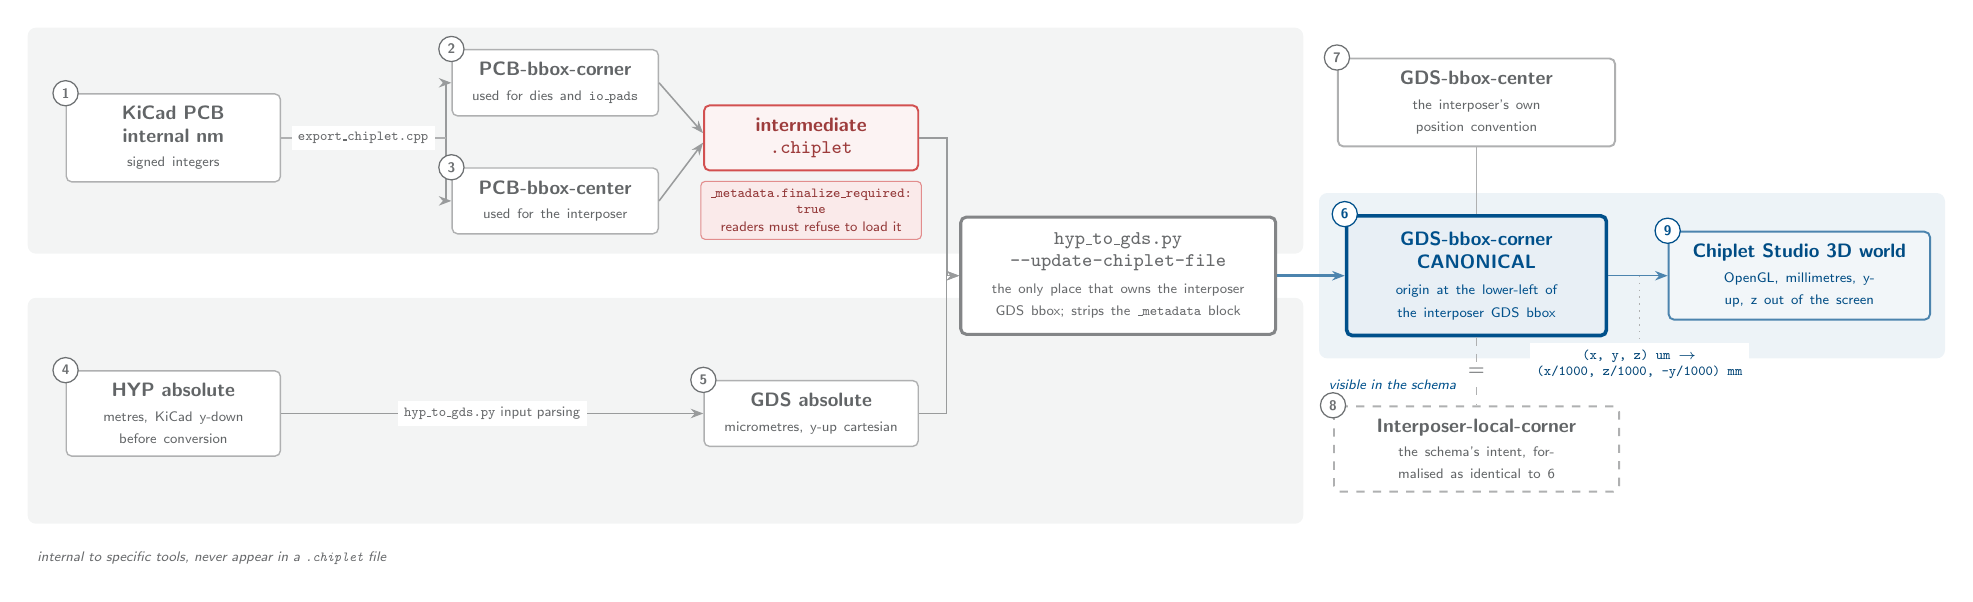
\begin{tikzpicture}[
    >=Stealth,
    adkframe/.style={
        rectangle, rounded corners=2pt,
        draw=IHPaccent!55, fill=white, line width=0.5pt,
        text width=23mm, align=center, inner sep=1.6mm,
        font=\sffamily\scriptsize, text=IHPaccent!90!black
    },
    adkmerge/.style={
        rectangle, rounded corners=2pt,
        draw=IHPaccent!85, fill=white, line width=1.1pt,
        text width=40mm, align=center, inner sep=2mm,
        font=\sffamily\scriptsize, text=IHPaccent!95!black
    },
    adkwarn/.style={
        rectangle, rounded corners=2pt,
        draw=IHPwarn, fill=IHPwarn!7, line width=0.7pt,
        text width=25mm, align=center, inner sep=1.6mm,
        font=\sffamily\scriptsize, text=IHPwarn!75!black
    },
    adkflag/.style={
        rectangle, rounded corners=1.5pt,
        draw=IHPwarn!65, fill=IHPwarn!12, line width=0.4pt,
        text width=26mm, align=center, inner sep=1mm,
        font=\sffamily\fontsize{4.8}{5.8}\selectfont, text=IHPwarn!70!black
    },
    adkcanon/.style={
        rectangle, rounded corners=2pt,
        draw=IHPfg, fill=IHPfg!9, line width=1.3pt,
        text width=30mm, align=center, inner sep=2mm,
        font=\sffamily\scriptsize, text=IHPfg
    },
    adkblue/.style={
        rectangle, rounded corners=2pt,
        draw=IHPfg!70, fill=IHPfg!5, line width=0.7pt,
        text width=28mm, align=center, inner sep=1.6mm,
        font=\sffamily\scriptsize, text=IHPfg!95!black
    },
    adknum/.style={
        circle, draw=#1, fill=white, line width=0.45pt,
        inner sep=0pt, minimum size=3.2mm,
        font=\sffamily\fontsize{5}{5}\selectfont\bfseries, text=#1
    },
    adkarrow/.style={-{Stealth[length=1.6mm]}, line width=0.55pt, color=IHPaccent!70},
    adklink/.style={line width=0.5pt, color=IHPaccent!55},
    adklbl/.style={
        font=\sffamily\fontsize{5}{6}\selectfont, text=IHPaccent!95!black,
        fill=white, inner sep=0.8mm, align=center
    },
    adkmono/.style={
        font=\ttfamily\fontsize{5}{6.4}\selectfont, text=IHPfg!85!black,
        fill=white, inner sep=0.8mm, align=center
    },
    adkbandlbl/.style={
        font=\sffamily\fontsize{5.2}{6.2}\selectfont\itshape, text=#1, align=left
    }
]

% ---------- background bands ----------
\fill[IHPaccent!8, rounded corners=3pt] (-1.85, 0.28) rectangle (14.35, 3.15);
\fill[IHPaccent!8, rounded corners=3pt] (-1.85,-3.15) rectangle (14.35,-0.28);
% Only frames 6 and 9 are visible from the schema, and both sit on the centre
% line, so the band is the middle strip and not the two outer halves.
\fill[IHPfg!7,    rounded corners=3pt] (14.55,-1.05) rectangle (22.50, 1.05);

\node[adkbandlbl=IHPaccent!95!black, anchor=north west] at (-1.85,-3.38)
    {internal to specific tools, never appear in a \texttt{.chiplet} file};
\node[adkbandlbl=IHPfg, anchor=north west] at (14.55,-1.20)
    {visible in the schema};

% ---------- upper track: the KiCad branch ----------
\node[adkframe, text width=24mm] (n1) at (0, 1.75)
    {\textbf{KiCad PCB internal nm}\\[0.3mm]{\tiny signed integers}};

\node[adkframe] (n2) at (4.85, 2.45)
    {\textbf{PCB-bbox-corner}\\[0.3mm]{\tiny used for dies and \texttt{io\_pads}}};

\node[adkframe] (n3) at (4.85, 0.95)
    {\textbf{PCB-bbox-center}\\[0.3mm]{\tiny used for the interposer}};

\node[adkwarn, text width=24mm] (nr) at (8.10, 1.75)
    {\textbf{intermediate \texttt{.chiplet}}};

\node[adkflag, anchor=north] at ([yshift=-1.2mm]nr.south)
    {\texttt{\_metadata.finalize\_required: true}\\[0.2mm]readers must refuse to load it};

% fork
\coordinate (fk) at (3.46, 1.75);
\draw[adkarrow] (fk) |- (n2.west);
\draw[adkarrow] (fk) |- (n3.west);
\draw[adklink] (n1.east) -- (fk);
\node[adklbl] at (2.41, 1.75) {\texttt{export\_chiplet.cpp}};

\draw[adkarrow] (n2.east) -- ([yshift=0.6mm]nr.west);
\draw[adkarrow] (n3.east) -- ([yshift=-0.6mm]nr.west);

% ---------- lower track: the geometry branch ----------
\node[adkframe, text width=24mm] (n4) at (0, -1.75)
    {\textbf{HYP absolute}\\[0.3mm]{\tiny metres, KiCad y-down before conversion}};

\node[adkframe, text width=24mm] (n5) at (8.10, -1.75)
    {\textbf{GDS absolute}\\[0.3mm]{\tiny micrometres, y-up cartesian}};

\draw[adkarrow] (n4.east) -- node[adklbl, pos=0.5]
    {\texttt{hyp\_to\_gds.py} input parsing} (n5.west);

% ---------- merge ----------
\node[adkmerge, text width=36mm] (mg) at (12.00, 0)
    {\textbf{\texttt{hyp\_to\_gds.py --update-chiplet-file}}\\[0.6mm]
     {\tiny the only place that owns the interposer GDS bbox;
      strips the \texttt{\_metadata} block}};

\draw[adkarrow] (nr.east) -- ++(0.35,0) |- (mg.west);
\draw[adkarrow] (n5.east) -- ++(0.35,0) |- (mg.west);

% ---------- canonical output ----------
\node[adkcanon, text width=29mm] (n6) at (16.55, 0)
    {\textbf{GDS-bbox-corner}\\[0.2mm]\textbf{CANONICAL}\\[0.5mm]
     {\tiny origin at the lower-left of the interposer GDS bbox}};

\draw[adkarrow, line width=0.9pt, color=IHPfg!70] (mg.east) -- (n6.west);

\node[adkblue, draw=IHPaccent!55, fill=white, text=IHPaccent!90!black,
      text width=32mm] (n7) at (16.55, 2.20)
    {\textbf{GDS-bbox-center}\\[0.3mm]{\tiny the interposer's own position convention}};

\node[adkblue, draw=IHPaccent!55, fill=white, text=IHPaccent!90!black,
      text width=33mm, dashed] (n8) at (16.55, -2.20)
    {\textbf{Interposer-local-corner}\\[0.3mm]{\tiny the schema's intent, formalised as identical to 6}};

\draw[adklink] (n6.north) -- (n7.south);
\draw[adklink, dashed] (n6.south) -- node[midway, fill=white, inner sep=0.5mm,
    font=\sffamily\scriptsize, text=IHPaccent!90!black] {$=$} (n8.north);

% ---------- final hop ----------
\node[adkblue, text width=30mm] (n9) at (20.65, 0)
    {\textbf{Chiplet Studio 3D world}\\[0.3mm]{\tiny OpenGL, millimetres, y-up, z out of the screen}};

\draw[adkarrow, color=IHPfg!70] (n6.east) -- (n9.west);
\draw[adklink, dotted] (18.62, 0) -- (18.62,-0.85);
\node[adkmono, anchor=north] at (18.62,-0.85)
    {(x, y, z) um $\rightarrow$\\[-0.2mm](x/1000, z/1000, -y/1000) mm};

% ---------- frame number badges ----------
\node[adknum=IHPaccent] at (n1.north west) {1};
\node[adknum=IHPaccent] at (n2.north west) {2};
\node[adknum=IHPaccent] at (n3.north west) {3};
\node[adknum=IHPaccent] at (n4.north west) {4};
\node[adknum=IHPaccent] at (n5.north west) {5};
\node[adknum=IHPfg]     at (n6.north west) {6};
\node[adknum=IHPaccent] at (n7.north west) {7};
\node[adknum=IHPaccent] at (n8.north west) {8};
\node[adknum=IHPfg]     at (n9.north west) {9};

\end{tikzpicture}
\end{document}
